\documentclass[12pt,letterpaper]{report}

\usepackage[margin=0.25in]{geometry}
\geometry{
  top=0.8in,            
  inner=1.0in,
  outer=1.0in,
  bottom=0.9in,
  headheight=4ex,       
  headsep=6.5ex,         
}

\setcounter{secnumdepth}{3}
\setcounter{tocdepth}{3}

\usepackage[utf8]{inputenc}
\usepackage[utf8]{vietnam}
\usepackage[english]{babel}
\usepackage{float}
\usepackage{xcolor}
\usepackage{verbatim}
\usepackage{charter}
\usepackage{amsmath}
\usepackage{appendix}
\usepackage{ragged2e}
\usepackage{array}
\usepackage{etoolbox}
\usepackage{fancyhdr}
\usepackage{booktabs}
\usepackage{arydshln}
\usepackage[format=hang,labelfont=bf]{caption}
\usepackage{subcaption}
\usepackage{enumitem}
\usepackage{amssymb}
\usepackage{graphicx}
\usepackage{mathtools}
\usepackage{multirow}
\usepackage{pdfpages}
\usepackage{subfiles}
\usepackage[compact]{titlesec}
\usepackage{stfloats}
\usepackage[style=ieee]{biblatex}
\usepackage{subfiles}
\usepackage[acronym]{glossaries}
\usepackage{gensymb}
\usepackage{algorithm}
\usepackage{algpseudocode}
\usepackage{nameref}
\usepackage[export]{adjustbox}

% UML diagram
\usepackage{plantuml}

\usepackage{hyperref}
\hypersetup{
    colorlinks=true,
    linkcolor=blue,
    filecolor=magenta,      
    urlcolor=cyan,
    pdftitle={Overleaf Example},
    pdfpagemode=FullScreen,
    }

\usepackage{listings}

\definecolor{codegreen}{rgb}{0,0.6,0}
\definecolor{codegray}{rgb}{0.5,0.5,0.5}
\definecolor{codepurple}{rgb}{0.58,0,0.82}
\definecolor{backcolour}{rgb}{0.95,0.95,0.92}

\lstdefinestyle{mystyle}{
    backgroundcolor=\color{backcolour},   
    commentstyle=\color{codegreen},
    keywordstyle=\color{magenta},
    numberstyle=\tiny\color{codegray},
    stringstyle=\color{codepurple},
    basicstyle=\ttfamily\footnotesize,
    breakatwhitespace=false,         
    breaklines=true,                 
    captionpos=b,                    
    keepspaces=true,                 
    numbers=left,                    
    numbersep=5pt,                  
    showspaces=false,                
    showstringspaces=false,
    showtabs=false,                  
    tabsize=1
}

\lstset{style=mystyle}

\lstdefinelanguage{JavaScript}{
  morekeywords={typeof, new, true, false, catch, function, return, null, catch, switch, var, if, in, while, do, else, case, break, setInterval, preventDefault, getElementById, ajax, serialize, get, done},
  morecomment=[s]{/*}{*/},
  morecomment=[l]//,
  morestring=[b]",
  morestring=[b]'
}

\addbibresource{datasheet_ref.bib}
\addbibresource{temp_ref.bib}

\title{PowerMeterOutline}
\author{Quan Dao Nguyen Anh}
\date{July 2023}

\begin{document}
\pagenumbering{roman}
\subfile{cover_page.tex}

\pagebreak

\tableofcontents
\listoffigures
\listoftables
\pagebreak
\pagenumbering{arabic}

\chapter{Introduction}
\pagebreak
\subfile{intro.tex}

\chapter{Circuit design}

\begin{figure}[!h]
  \centerline{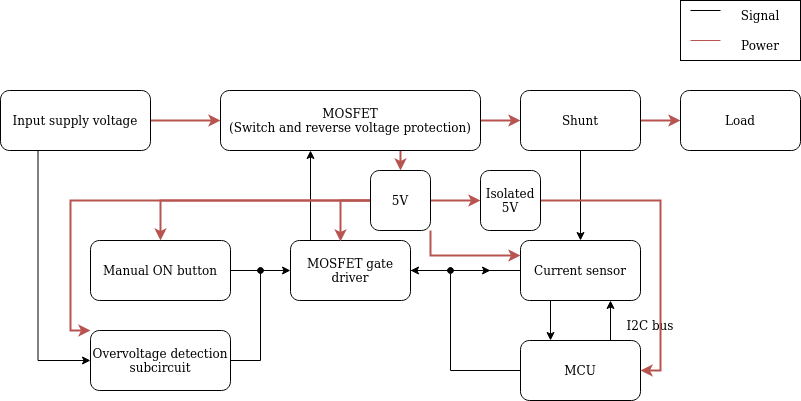
\includegraphics[width=\linewidth]{media/circuit_diagram.drawio.png}}
  \caption{Subcircuits connection: power and signal.}
  \label{fig:Circuit flowchart}
\end{figure}

\justify
In this chapter, the following aspects of designing this project's circuit are discussed:
\begin{enumerate}
  \item MOSFET selection.
  \item MOSFET driver.
  \item Power rail.
  \item Latch and overvoltage detection subcircuit.
  \item Sensor and MCU.
\end{enumerate}

\pagebreak
\subfile{circuit_design/MOSFET_selection.tex}
\pagebreak
\subfile{circuit_design/MOSFET_driver.tex}
\pagebreak
\subfile{circuit_design/power_rail.tex}
\pagebreak
\subfile{circuit_design/latch_circuit.tex}
\pagebreak
\subfile{circuit_design/sensor_mcu.tex}

\chapter{PCB layout}
\justify
\begin{figure}[!h]
  \centerline{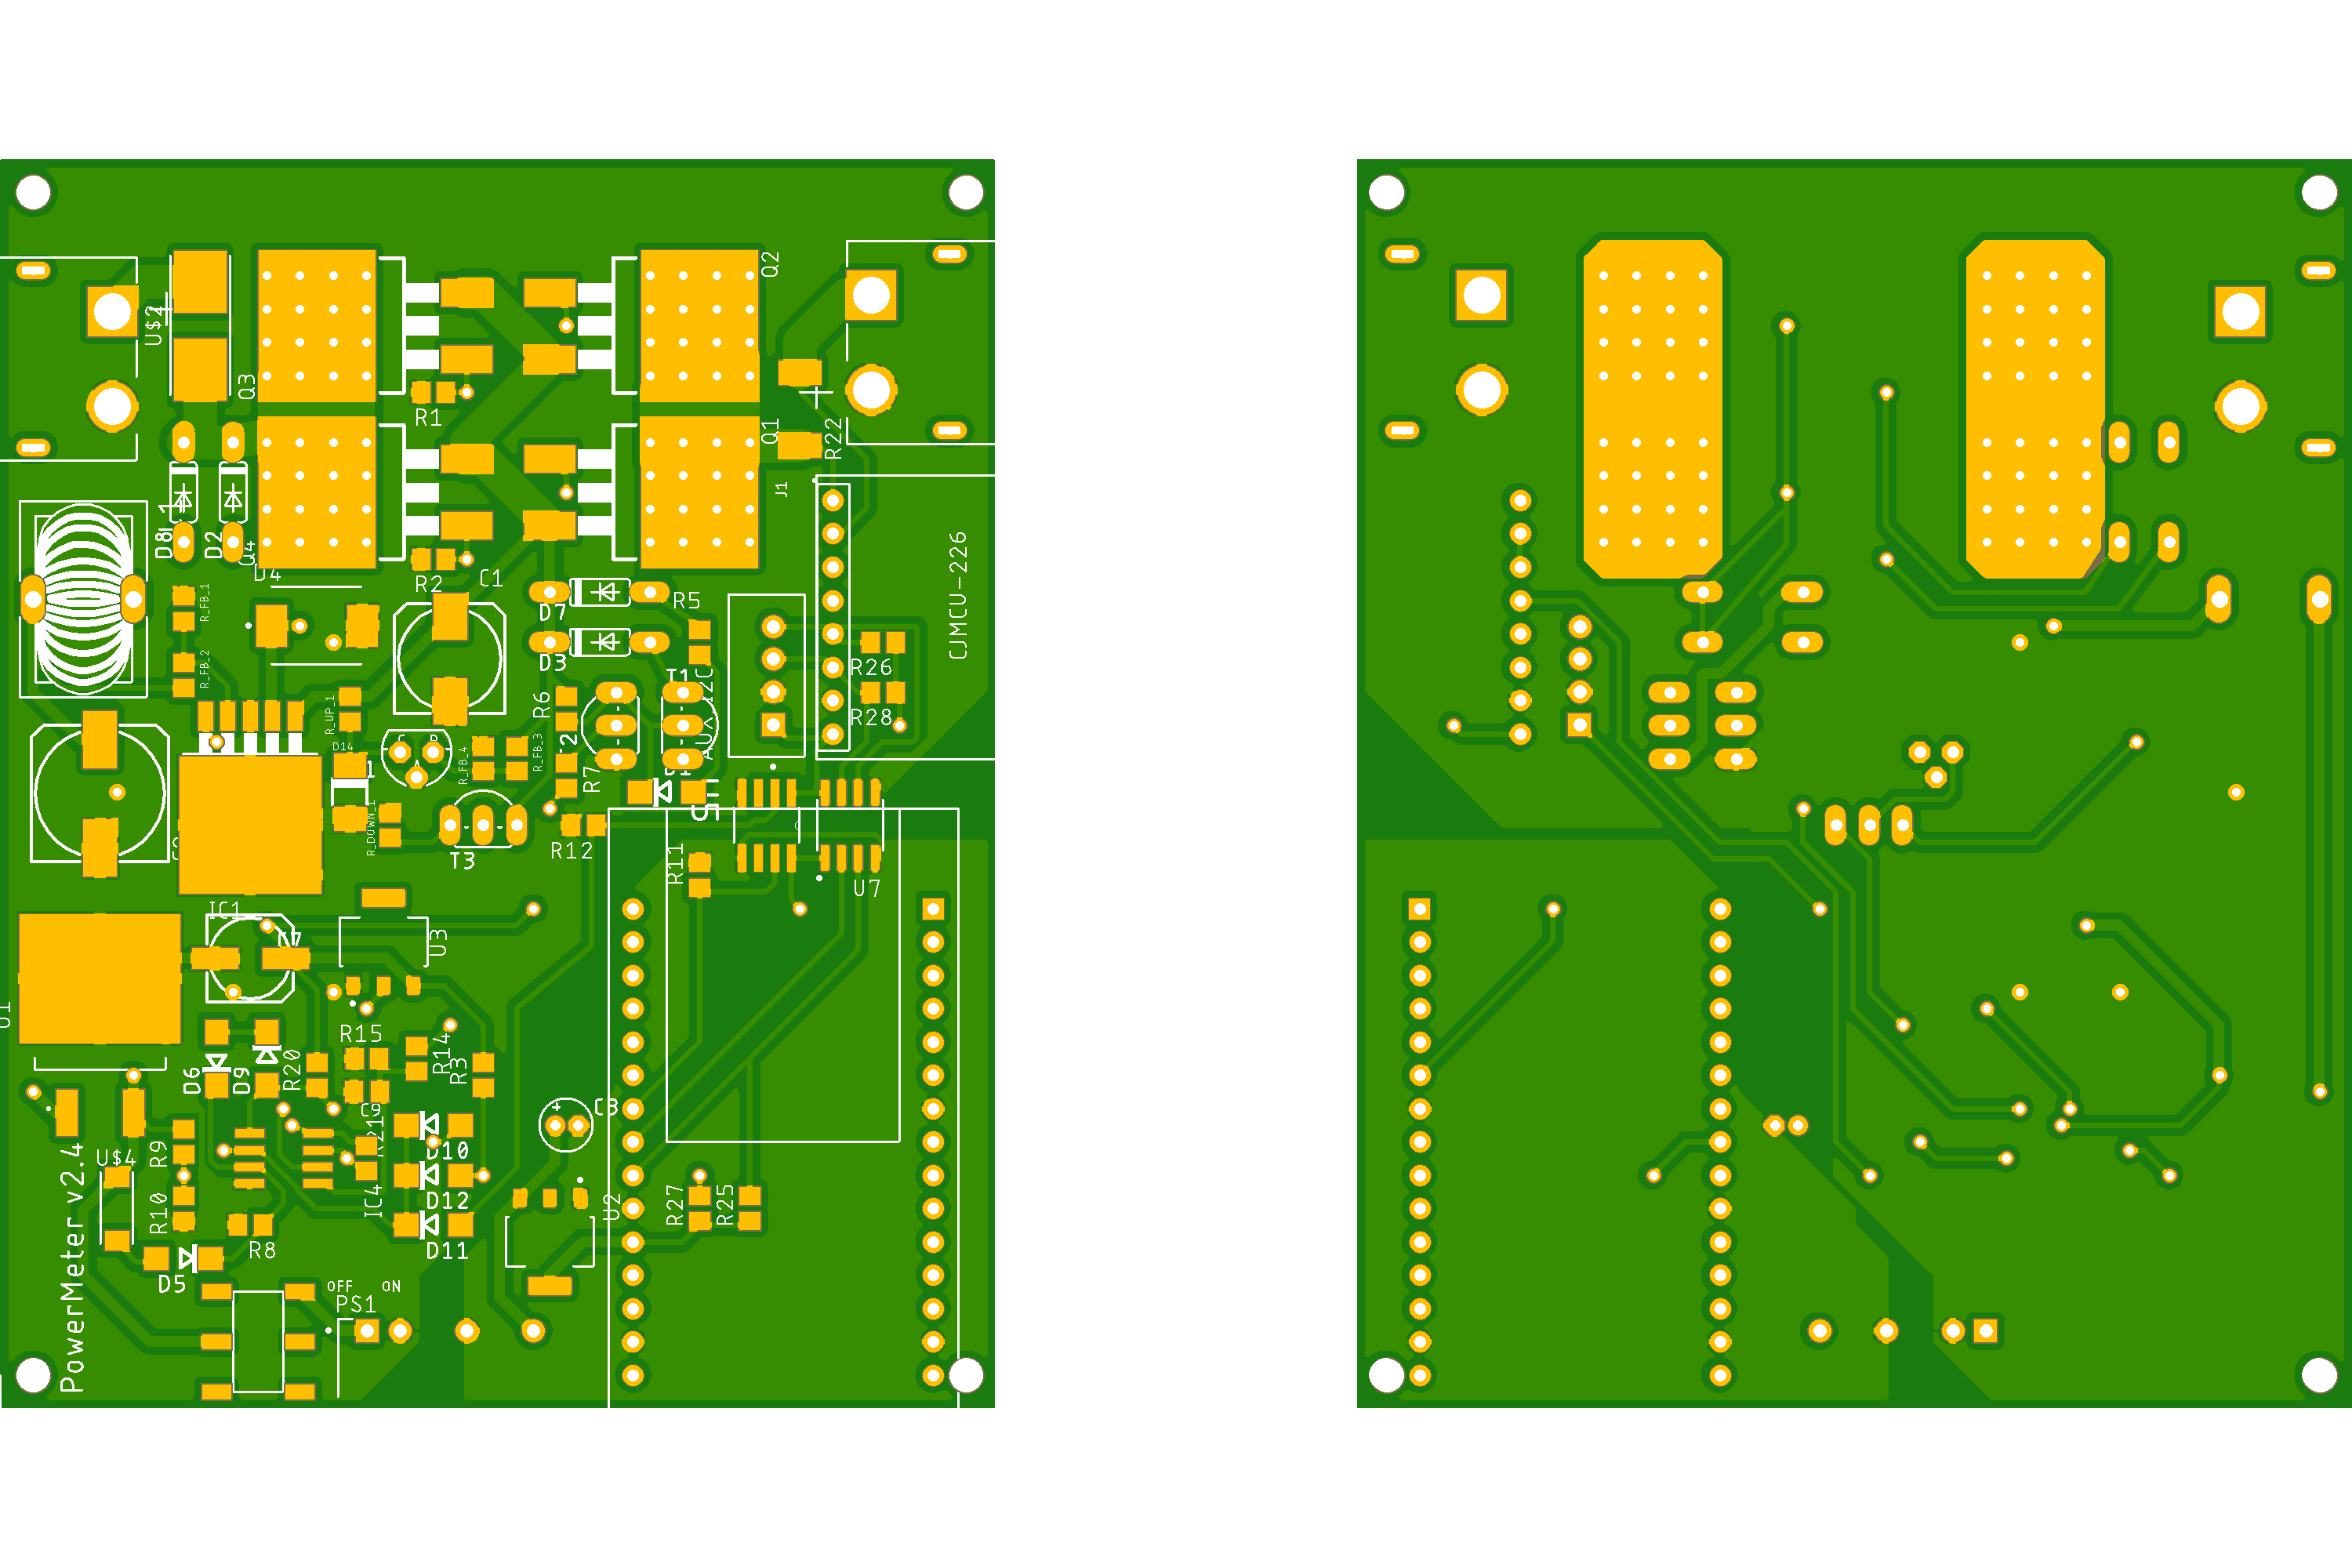
\includegraphics[width=\linewidth]{media/power_meter_pcb_v2_2.png}}
  \caption{Top (left) and bottom layer of the PCB layout.}
\end{figure}
In this chapter, the following key design points of the PCB layout are discussed:
\begin{itemize}
  \item Thermal via for TO-263/D2PAK footprint.
  \item Amass XT60PW connector.
\end{itemize}
\pagebreak
\subfile{circuit_design/pcb_layout.tex}

\chapter{Firmware}
\justify
In this chapter, FreeRTOS is first discussed as it is an important component in the firmware of the MCU. Then, the firmware flowchart is discussed. The firmware of the MCU is built by running asynchronous tasks utilizing FreeRTOS with limited shared resources to limit bottlenecking.
\pagebreak
\subfile{firmware/firmware.tex}

\chapter{Application}
\justify
In this chapter, the application design is discussed. The application is built using the Model-View-Vontroller design pattern. 

\begin{figure}[!h]
  \centerline{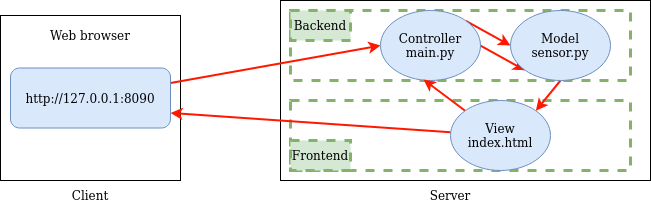
\includegraphics[width=\linewidth]{media/mvc_modified.drawio.png}}
  \caption{Model-View-Controller diagram.}
  \label{fig:application_flowchart}
\end{figure}

\pagebreak
\subfile{application/application.tex}

\chapter{Result}
After evaluating the design, the following observations are made:
\begin{itemize}
  \item The proposed gate driver design and the power rail fails to meet their desired behaviour. These problems are discussed in details in Section \ref{sec:result_gate_driver} and \ref{sec:result_power_rail}.
  \item The latch subcircuit design does not account for attempt at closing the switch after occurence of a fault. Section \ref{sec:result_latch_circuit} discusses this issue and proposes a possible improvements.
  \item The communication between the firmware and application, as well as data visualization are discussed in Section \ref{sec:result_fw_app}.
\end{itemize}

\pagebreak
\subfile{result.tex}

\chapter{Conclusion}
\justify
Despite the issues with the gate driver and the power rail, the goals set out by the thesis are still achieved. With the pure resistive test load, the power monitor is able to operate well within the maximum ratings. The application allows the user to disconnect the load from the power supply at a click of a mouse, configure the desired protection threshold, and monitor the operating voltage and current traces of the connected load. To be able to use with other load (capacitive and/or inductive), the large $dv/dt$ at switch turn-off needs to be addressed. To make the device more portable, an alternative isolated DC-DC converter to the B0505S-2WR2 must be investigated.


\printbibliography

\end{document}
